\documentclass[a4paper, 10pt, twoside]{article}

\usepackage[top=1in, bottom=1in, left=1in, right=1in]{geometry}
\usepackage[utf8]{inputenc}
\usepackage[spanish, es-ucroman, es-noquoting]{babel}
\usepackage{setspace}
\usepackage{fancyhdr}
\usepackage{lastpage}
\usepackage{amsmath}
\usepackage{amsfonts}
\usepackage{amsthm}
\usepackage{verbatim}
\usepackage{graphicx}
\usepackage{float}
\usepackage{enumitem} % Provee macro \setlist
\usepackage{tabularx}
\usepackage{multirow}
\usepackage{hyperref}
\usepackage{multicol}
\usepackage[toc, page]{appendix}


%%%%%%%%%% Configuración de Fancyhdr - Inicio %%%%%%%%%%
\pagestyle{fancy}
\thispagestyle{fancy}
\lhead{Trabajo Práctico 1 · Ingeniería de Software I}
\rhead{Aboy · Almansi · Canay · Contrufo · Decroix}
\renewcommand{\footrulewidth}{0.4pt}
\cfoot{\thepage /\pageref{LastPage}}

\fancypagestyle{caratula} {
   \fancyhf{}
   \cfoot{\thepage /\pageref{LastPage}}
   \renewcommand{\headrulewidth}{0pt}
   \renewcommand{\footrulewidth}{0pt}
}
%%%%%%%%%% Configuración de Fancyhdr - Fin %%%%%%%%%%


%%%%%%%%%% Miscelánea - Inicio %%%%%%%%%%
% Evita que el documento se estire verticalmente para ocupar el espacio vacío
% en cada página.
\raggedbottom

% Deshabilita sangría en la primer línea de un párrafo.
\setlength{\parindent}{0em}

% Separación entre párrafos.
\setlength{\parskip}{0.5em}

% Separación entre elementos de listas.
\setlist{itemsep=0.5em}

% Asigna la traducción de la palabra 'Appendices'.
\renewcommand{\appendixtocname}{Apéndices}
\renewcommand{\appendixpagename}{Apéndices}
%%%%%%%%%% Miscelánea - Fin %%%%%%%%%%


%%%%%%%%%% Insertar diagrama - Inicio %%%%%%%%%%
\newcommand{\diagramav}[1]{
  \includegraphics[type=png,ext=.png,read=.png,width=16cm]{diagramas/#1}
}

\newcommand{\diagramah}[1]{
  \includegraphics[type=png,ext=.png,read=.png,height=16cm,angle=90]{diagramas/#1}
}
%%%%%%%%%% Insertar diagrama - Fin %%%%%%%%%%

\begin{document}


%%%%%%%%%%%%%%%%%%%%%%%%%%%%%%%%%%%%%%%%%%%%%%%%%%%%%%%%%%%%%%%%%%%%%%%%%%%%%%%
%% Carátula                                                                  %%
%%%%%%%%%%%%%%%%%%%%%%%%%%%%%%%%%%%%%%%%%%%%%%%%%%%%%%%%%%%%%%%%%%%%%%%%%%%%%%%


\thispagestyle{caratula}

\begin{center}


\includegraphics[height=2cm]{DC.png} 
\hfill

\includegraphics[height=2cm]{UBA.jpg} 

\vspace{2cm}

Departamento de Computación,\\
Facultad de Ciencias Exactas y Naturales,\\
Universidad de Buenos Aires

\vspace{4cm}

\begin{Huge}
Trabajo Práctico 1
\end{Huge}

\vspace{0.5cm}

\begin{Large}
Ingeniería de Software I
\end{Large}

\vspace{1cm}

Segundo Cuatrimestre de 2014

\vspace{4cm}

\begin{Large}
Grupo 4
\end{Large}

\vspace{0.5cm}

\begin{tabular}{|c|c|c|}
\hline
Nombre y Apellido & LU & E-mail\\
\hline
Santiago Aboy Solanes & 175/12 & santiaboy2@hotmail.com\\
Emilio Almansi & 674/12 & ealmansi@gmail.com\\
Federico Canay & 250/12 & fcanay@hotmail.com\\
Maximiliano Contrufo & 336/12 & maxicontru@gmail.com\\
Facundo Decroix & 842/11 & fndecroix92@hotmail.com\\
\hline
\end{tabular}

\end{center}

\newpage


%%%%%%%%%%%%%%%%%%%%%%%%%%%%%%%%%%%%%%%%%%%%%%%%%%%%%%%%%%%%%%%%%%%%%%%%%%%%%%%
%% Índice                                                                    %%
%%%%%%%%%%%%%%%%%%%%%%%%%%%%%%%%%%%%%%%%%%%%%%%%%%%%%%%%%%%%%%%%%%%%%%%%%%%%%%%


\tableofcontents

\newpage


%%%%%%%%%%%%%%%%%%%%%%%%%%%%%%%%%%%%%%%%%%%%%%%%%%%%%%%%%%%%%%%%%%%%%%%%%%%%%%%
%% Introducción                                                              %%
%%%%%%%%%%%%%%%%%%%%%%%%%%%%%%%%%%%%%%%%%%%%%%%%%%%%%%%%%%%%%%%%%%%%%%%%%%%%%%%


\section{Introducción}

El CEO de TecnoTaxi nos contactó para solicitarnos crear un sistema. Nuestro objetivo es realizar un sistema para la automatización de las solicitudes de taxis de los pasajeros y la coordinación de los viajes con los taxistas. Antes de realizar el sistema en sí, vamos a proporcionar la mayor cantidad de información posible respecto de cómo nuestra propuesta va a ayudar a cumplir con los objetivos planteados. En particular, vamos a proporcionar un diagrama de contexto y un diagrama de objetivos.

%%%%%%%%%%%%%%%%%%%%%%%%%%%%%%%%%%%%%%%%%%%%%%%%%%%%%%%%%%%%%%%%%%%%%%%%%%%%%%%
%% Escenarios hipotéticos                                                    %%
%%%%%%%%%%%%%%%%%%%%%%%%%%%%%%%%%%%%%%%%%%%%%%%%%%%%%%%%%%%%%%%%%%%%%%%%%%%%%%%

\section{Escenarios hipotéticos}

Los siguientes escenarios ilustran de manera informal situaciones representativas del funcionamiento esperado del sistema.

\subsection{Escenario 1}

Alicia necesita viajar hasta el consultorio de su dentista y elige la moderna empresa TecnoTaxi para solicitar un taxi. Como ella está al día en cuestiones tecnológicas, tiene instalada la aplicación de la empresa en su smartphone y desea realizar la solicitud mediante la misma.

Alicia inicia el proceso de solicitud en la aplicación, ingresando la dirección de origen del viaje, la dirección destino y sus preferencias: un auto moderno. El sistema le muestra mediante la aplicación una lista de opciones de diferentes taxistas que cumplen su pedido y ella elige a Florencia, que maneja un Chevrolet último modelo.

\subsection{Escenario 2}

Omar pidió un taxi para las 17:00hs, para ir a visitar a su suegra. Afortunadamente, ella lo llama para postergar el encuentro. Omar usa su teléfono para avisar a TecnoTaxi y cancelar su viaje.

\subsection{Escenario 3}

Micaela realizó un viaje durante el cual el conductor le realizó múltiples insinuaciones. Ni bien terminó su viaje, dio una calificación de una estrella al conductor y publicó un comentario para que no le pase a nadie más.

\subsection{Escenario 4}

Cada vez que Lucas viaja con su taxista preferido, Roberto, llega a su destino con una sonrisa en su cara. Roberto es un gran comediante amateur. Lucas decide calificar a Roberto positivamente para que todos sepan lo buena persona que es.

\subsection{Escenario 5}

Alfredo desea ir a visitar a su tía, que vive en Boedo. Él es un pasajero usual de TecnoTaxi, por lo que tiene ya descargada en su smartphone la aplicación móvil de viajes. Al abrir la aplicación, la misma le indica que no se puede encontrar una conexión a internet, por lo que deberá comunicarse por otros medios, sugiriendo la página web de la empresa y el número de teléfono para comunicarse por vía telefónica. Alfredo se dirige entonces a su computadora para solicitar el taxi vía web. Al abrir el navegador web, su página de inicio no carga correctamente. Sorprendido, Alfredo tipea la dirección de la página web indicada por la aplicación, pero su computadora tampoco logra cargarla: no tiene acceso a internet. Indignado por el pésimo servicio de internet que brindan tanto el servidor de internet que utiliza en su casa como el del celular, Alfredo decide hacer su pedido de viaje por teléfono. Llama a la línea telefónica de la empresa de taxis y es atendido por una cordial operadora, y realiza el pedido por 
este medio.

\subsection{Escenario 6}

Ronaldo va a su masajista todos los martes a las 15:00hs. Necesita un taxi para llegar a horario y no perder la sesión de masajes. Ronaldo llama a TecnoTaxi y programa un viaje de rutina para las 14:30hs de todos los martes. Desde ese momento y hasta el día presente, Ronaldo no perdió ninguna sesión de masajes.


%%%%%%%%%%%%%%%%%%%%%%%%%%%%%%%%%%%%%%%%%%%%%%%%%%%%%%%%%%%%%%%%%%%%%%%%%%%%%%%
%% Desarrollo                                                                %%
%%%%%%%%%%%%%%%%%%%%%%%%%%%%%%%%%%%%%%%%%%%%%%%%%%%%%%%%%%%%%%%%%%%%%%%%%%%%%%%


\section{Desarrollo}

\subsection{Requerimientos}

\begin{enumerate}
 \item Brindar a los usuarios esperando un taxi la información de donde se encuentra el mismo y cual es el tiempo de demora.
 \item Poder calificar los viajes, para que otros usuarios puedan elegir no viajar con determinado chofer.
 \item Que el cliente pueda elegir el coche con el que viajar.
 \item Que a los taxistas solo le ofrezca la operadora viajes dentro de su alcance.
 \item Brindar al usuario una opción para cancelar el viaje.
 \item Que los pasajeros puedan solicitar un viaje vía web o móvil.
 \item Seguir aportando servicio a los pasajeros sin acceso a Internet o a la tecnología.
 \item Que los pasajeros puedan planificar viajes de rutina.
 \item Automatizar la asistencia al pasajero en la elección de auto/chofer.
 \item Proveer un conjunto de estadísticas para los directivos.
\end{enumerate}



%%%%%%%%%%%%%%%%%%%%%%%%%%%%%%%%%%%%%%%%%%%%%%%%%%%%%%%%%%%%%%%%%%%%%%%%%%%%%%%
%% Diagrama de Contexto                                                      %%
%%%%%%%%%%%%%%%%%%%%%%%%%%%%%%%%%%%%%%%%%%%%%%%%%%%%%%%%%%%%%%%%%%%%%%%%%%%%%%%

\appendix
\section{Diagrama de contexto}

  \begin{figure}[H]
    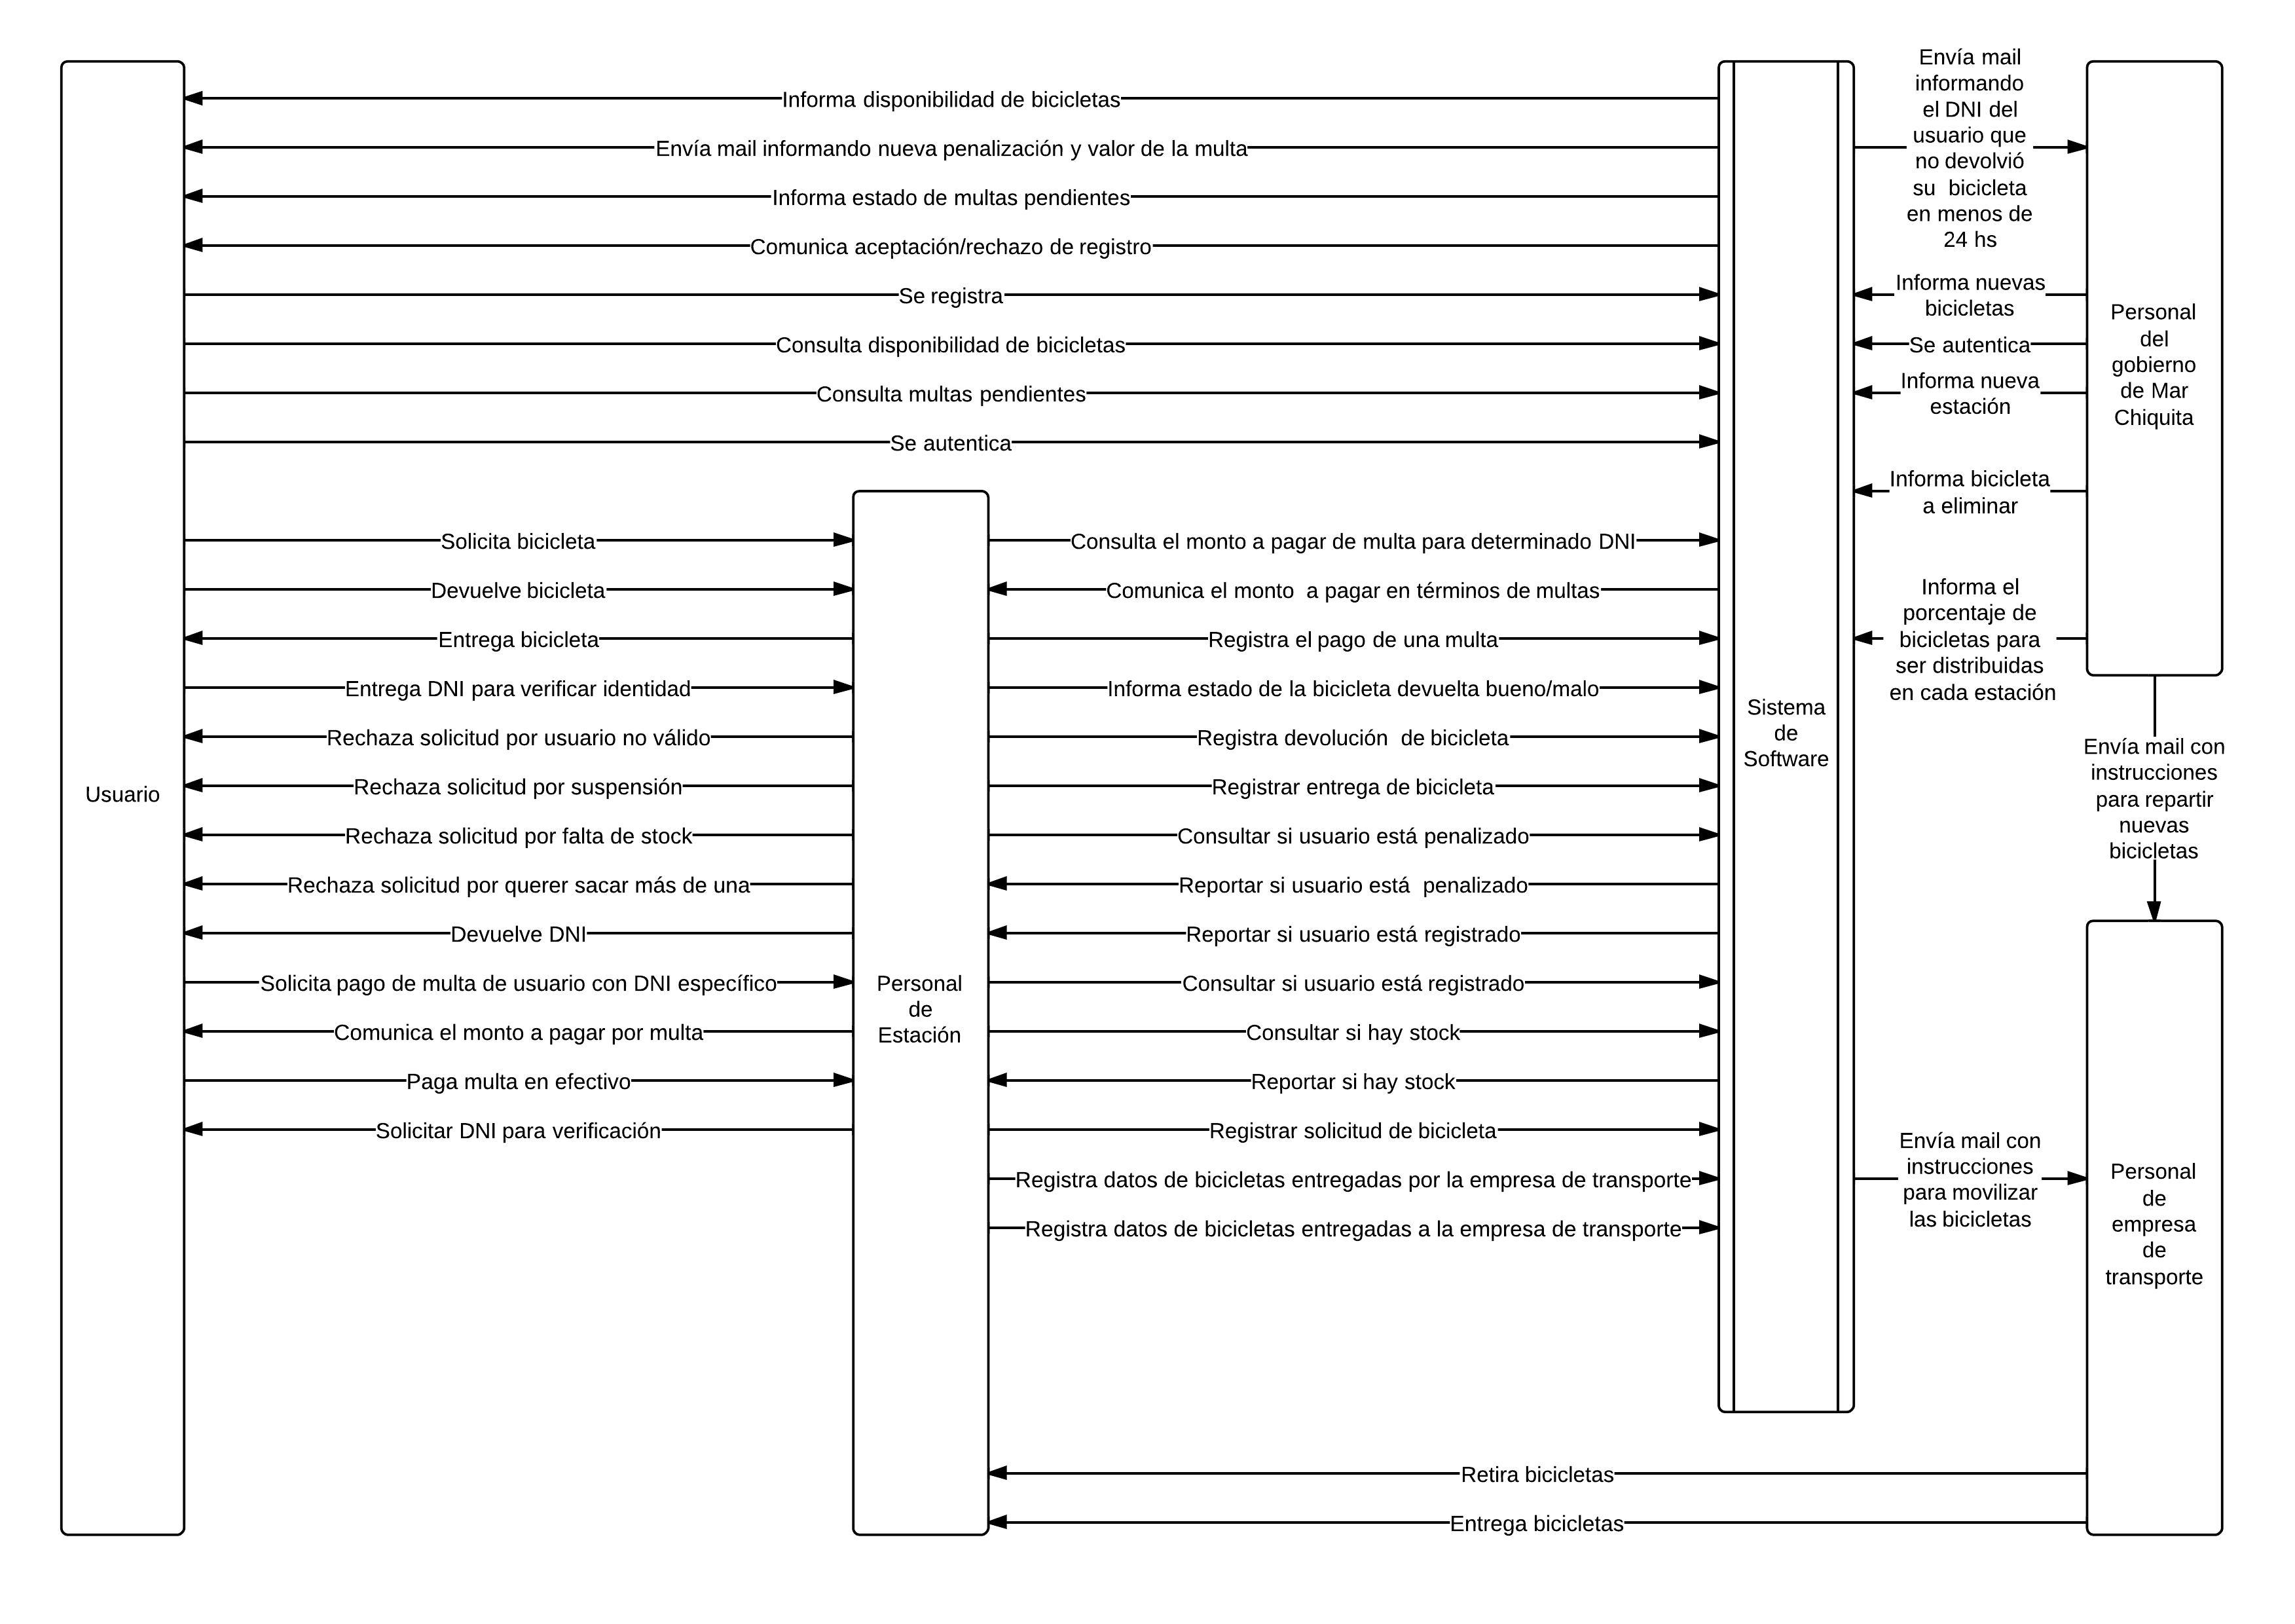
\includegraphics[height=15cm,angle=90]{diagramas/contexto.png}
  \end{figure}

\subsection{Actores}

A continuación, vamos a explicar los distintos actores que están presentes en nuestro diagrama de contexto.

  \begin{enumerate}
    \item \textbf{Sistema:} El sistema a crear.
    \item \textbf{Aplicación Móvil:} Aplicación móvil con la cual los usuarios pueden pedir taxis, calificar taxistas, etc. Esta aplicación es externa a nuestro sistema.
    \item \textbf{Aplicación Web:} Aplicación web con la cual los usuarios pueden pedir taxis, calificar taxistas, etc. Esta aplicación es externa a nuestro sistema.
    \item \textbf{Operador Telefónico/ de radio:} Empleado de la empresa encargado de atender teléfonos, y hablar con taxistas para coordinar viajes.
    \item \textbf{Cliente No Registrado:} Cualquier persona que se comunique vía telefónica, sin importar si tiene un usuario registrado en el sistema o no.
    \item \textbf{Cliente Registrado:} Cualquier persona que se haya registrado previamente en el sistema. Registrando un nombre de usuario y una contraseña.
    \item \textbf{Directivos:} Empleados de la empresa encargados de dirigir la misma.
    \item \textbf{Taxista:} Un empleado de la empresa que maneja taxis.
    \item \textbf{GPS:} Sistema de navegación y localización mediante satélites.
  \end{enumerate}

\subsection{Fenómenos destacados}

A continuación, vamos a enumerar y explicar algunos fenómenos que creemos que vale la pena aclarar.

   \begin{enumerate}
     \item \textbf{Informar Modificación de Estado:} Por Informar Modificación de Estado nos referimos a que el taxista informa si surgió un contratiempo, como por ejemplo que pinchó una goma.
     \item \textbf{Hacer Pedido:} Por Hacer Pedido nos referimos a que el cliente indica desde donde, a donde quiere ir y cuáles son sus preferencias (si las tiene).
     \item \textbf{Brindar Opciones:} Por Brindar Opciones nos referimos a que las aplicaciones le indican al cliente cuáles son las mejores opciones de taxistas dado su pedido.
     \item \textbf{Informar llegada y coordinar encuentro:} Por Informar llegada y coordinar encuentro nos referimos a que el taxista le avisa al cliente que llegó a la dirección coordenada para empezar el viaje.
     \item \textbf{Calificar:} Por Calificar nos referimos a que el cliente califica a un cierto taxista, con una cierta cantidad de estrellas (1-5).
  \end{enumerate}
 
 \subsection{Aclaraciones}
 
 Cabe resaltar que el optar por dejar la Aplicación M\'ovil y la Aplicación Web por fuera del sistema, deja de ser parte del producto que vamos a realizar y pasa a hacer algo que se supone que se consigue.
 
\newpage

%%%%%%%%%%%%%%%%%%%%%%%%%%%%%%%%%%%%%%%%%%%%%%%%%%%%%%%%%%%%%%%%%%%%%%%%%%%%%%%
%% Modelo de Objetivos                                                       %%
%%%%%%%%%%%%%%%%%%%%%%%%%%%%%%%%%%%%%%%%%%%%%%%%%%%%%%%%%%%%%%%%%%%%%%%%%%%%%%%


\section{Modelo de objetivos}

%TODO agregar el diagrama en si

\newpage

\subsection{Objetivos de alto nivel}

%TODO terminar

En esta sección vamos a explicar un poco los objetivos de alto nivel, y por qué están en esas posiciones en el diagrama.

\begin{itemize}

\item \textbf{Conocer estadísticas acerca del ambiente del trabajo, permite aumentar las ganancias}: Al conocer las estadísticas del ambiente del trabajo, puedo obtener un mejor conocimiento del medio. Esto permite podes aprovechar mejor el capital, incurriendo en mayores ingresos y/o menores ingresos.

\end{itemize}


\subsection{Objetivos blandos}

En esta sección vamos a hablar de los \emph{o-refinamientos} del diagrama de objetivos y de cuáles son los objetivos blandos que utilizamos para compararlos.

\begin{itemize}
\item Lograr darse a conocer

  De este objetivo surge un \emph{o-refinamiento} que deriva en los siguientes objetivos:
  \begin{enumerate}
    \item Lograr armar campaña publicitaria
    \item Lograr estar presente en las redes sociales
  \end{enumerate}
	
  Para ponderar estas opciones del \emph{o-refinamiento} consideramos los siguientes objetivos blandos:
  \begin{enumerate}
    \item Efectividad en el corto plazo (menos de 3 meses)
      
      En este caso ambos objetivos aportan positivamente. Sin embargo nos parece que el primero es aún más efectivo a corto plazo que el segundo, ya que consideramos que una campaña publicitaria tiene un alcance más veloz que el de las redes sociales.

    \item Disminuir costo en el corto plazo (menos de 3 meses) %mediano plazo no hay diferencias asi que no hay objetivos blandos al respecto
      
      Creemos que ambos objetivos aportan negativamente a este objetivo ya que involucran gastos a la empresa. Sin embargo creemos que el primer objetivo es el que va más en contra de este objetivo ya que es más costosa una campaña publicitaria que estar presente en redes sociales.
    
    \item Disminuir costo en el largo plazo (mas de 1 año)
      
      Nuevamente ambos objetivos aportan negativamente. Pero creemos que a largo plazo estar presente en las redes sociales será más costoso que hacer una campaña publicitaria, la cual se paga sólo una vez.
  \end{enumerate}

\item Lograr proveer servicios novedosos
  
  En este caso el \emph{o-refinamiento} deriva en los siguientes objetivos:
  \begin{enumerate}
    \item Lograr organizar automáticamente los viajes
    \item Lograr gestionar eventualidades del viaje
    \item Lograr proveer ubicación de taxi durante la espera
    \item Lograr programar viajes de rutina
  \end{enumerate}
  
  En este caso pensamos los siguientes objetivos blandos relacionados:
  
  \begin{enumerate}
    \item Menos trabajo (en el sentido de menos cosas para hacer)

      \emph{Aclaración:} de algún modo este objetivo blando tiene mucho que ver con la idea de automatizar el sistema; es decir que haya menos tareas que tengan que ser realizadas por seres humanos y en cambio las realicen sistemas automáticos.
	
      A este objetivo blando aporta positivamente el primero de los objetivos mencionados, mientras que los demás no lo hacen ya que especifican funcionalidades en vez de automatizar las existentes.
      
    \item Opciones más convenientes para el pasajero
      
      Todos los objetivos planteados aportan positivamente a este objetivo blando pero creemos que los últimos dos objetivos mencionados aportan más ya que afectan directamente al cliente (en cuanto a cuantas veces tiene que gestionar pedidos, en el caso de los viajes de rutina; y en cuanto a poder organizarse mejor en función al tiempo de espera en el caso de proveer la ubicación del taxi). En cambio los otros dos objetivos no necesariamente repercuten de manera positiva en el cliente (por ejemplo si no surgen eventualidades en el viaje).
  \end{enumerate}

\item Lograr comunicarse con el cliente
  
  En este caso el \emph{o-refinamiento} deriva en los siguientes objetivos:
  
  \begin{enumerate}
    \item Lograr comunicarse vía aplicación web
    \item Lograr comunicarse vía aplicación móvil
  \end{enumerate}
  
  Surgieron los siguientes objetivos blandos:
  
  \begin{enumerate}
    \item Mayor llegada a los clientes

      Ambos objetivos aportan positivamente; sin embargo creemos que el primero aporta más ya que es mayor la cantidad de gente que puede tener acceso al servicio web que la que tiene acceso a un dispositivo móvil con el que pueda usar la aplicación.
      
    \item Comodidad para el pasajero
	
      En este caso también ambos objetivos aportan positivamente, pero creemos que el que brinda más comodidad es el segundo objetivo ya que en general el dispositivo móvil se suele brindar un acceso más directo (suele estar encendido, no hace falta abrir primero un navegador web, etc).
  \end{enumerate}
  
\item Lograr comunicarse con el taxista
  
  Esta vez el \emph{o-refinamiento} esta compuesto por los siguientes objetivos:
  
  \begin{enumerate}
    \item Lograr comunicarse vía aplicación web
    \item Lograr comunicarse vía radio
  \end{enumerate}
  
  Pensamos en el siguiente objetivo blando
  
  \begin{enumerate}
  
  \item Comodidad para el taxista
  
      En este caso creemos que el primer objetivo aporta negativamente ya que para utilizar la aplicación móvil el taxista deberá frenar su vehículo. En cambio la radio es un método más fácil de utilizar cuando se esta manejando.
  \end{enumerate}

\item Lograr aumentar el tamaño de la flota
  
  El \emph{o-refinamiento} esta compuesto por los siguientes objetivos:
  
  \begin{enumerate}
    \item Lograr fácil adopción de los sistemas de la empresa para el taxista
    \item Lograr anuncios de viajes menos invasivos para el taxista 
    \item Mantener garantías de menor cancelación sin aviso
  \end{enumerate}
  
  Pensamos en el siguiente objetivo blando
  
  \begin{enumerate}
    \item Mejorar condiciones laborales
  
      Todos los objetivos aportan de manera positiva a este objetivo. Pero creemos que el tercer objetivo es el que más aporta, ya que creemos que lo que más le molesta a un taxista es que le cancelen sin aviso lo cual puede hacer que recorra un trayecto innecesario y que no levante otros posibles pasajeros.
  \end{enumerate}
\end{itemize}

\end{document}
